%%%%%%%%%%%%%%%%%%%%%%%%%%%%%%%%%%%%%%%%%%%%%%%%%%%%%%%%%%%%%%%%%%%%%%%%%%%%%%%%
\documentclass[twocolumn]{revtex4}

%%%%%%%%%%%%%%%%%%%%%%%%%%%%%%%%%%%%%%%%%%%%%%%%%%%%%%%%%%%%%%%%%%%%%%%%%%%%%%%%
% Note that comments begin with a "%" and are not turned into text in the .pdf
% document.
%%%%%%%%%%%%%%%%%%%%%%%%%%%%%%%%%%%%%%%%%%%%%%%%%%%%%%%%%%%%%%%%%%%%%%%%%%%%%%%%

%%%%%%%%%%%%%%%%%%%%%%%%%%%%%%%%%%%%%%%%%%%%%%%%%%%%%%%%%%%%%%%%%%%%%%%%%%%%%%%%
% Include some extra packages.
%%%%%%%%%%%%%%%%%%%%%%%%%%%%%%%%%%%%%%%%%%%%%%%%%%%%%%%%%%%%%%%%%%%%%%%%%%%%%%%%
\usepackage[]{graphicx}
%%%%%%%%%%%%%%%%%%%%%%%%%%%%%%%%%%%%%%%%%%%%%%%%%%%%%%%%%%%%%%%%%%%%%%%%%%%%%%%%

%%%%%%%%%%%%%%%%%%%%%%%%%%%%%%%%%%%%%%%%%%%%%%%%%%%%%%%%%%%%%%%%%%%%%%%%%%%%%%%%
\begin{document}

%%%%%%%%%%%%%%%%%%%%%%%%%%%%%%%%%%%%%%%%%%%%%%%%%%%%%%%%%%%%%%%%%%%%%%%%%%%%%%%%
\title{
\bf Predicting the Weather
}

\author{N.~Pettiway}
\affiliation{Siena College, Loudonville, NY}

\date{\today}

\begin{abstract}

   {\it  The objective of this project was to predict the odds that it rains only one day in a month, the odds that it rains at least 8 days in a month, the odds that there at least ten centimeters of rain in a given month, making a histogram of this data, finding the average amount of rain fall in a month, and lastly, finding the uncertainty of the predictions. In order to make these predictions, I used the Monte Carlo approach. The odds that it will rain one day and only day in a given month is between 0.85\%  and  0.96\%, an average of {\bf 0.91\%}. The odds that it will rain at least eight days in a given month is between 0.74\% and 0.81\% , an average of {\bf 0.78\%}. I was able to create a historgram from the data from the rainfall amounts, unfortunately I did not make it that far in this experiment to find out the odds of at least ten centimeters of rain fall in a given month, the average amount of rain fall in any given month, or the uncertainty of these predictions. I will continue working on this data and present another document in the near future.}  
   
\end{abstract}

\maketitle
%%%%%%%%%%%%%%%%%%%%%%%%%%%%%%%%%%%%%%%%%%%%%%%%%%%%%%%%%%%%%%%%%%%%%%%%%%%%%%%%

%%%%%%%%%%%%%%%%%%%%%%%%%%%%%%%%%%%%%%%%%%%%%%%%%%%%%%%%%%%%%%%%%%%%%%%%%%%%%%%%
\section{\bf Introduction}
%%%%%%%%%%%%%%%%%%%%%%%%%%%%%%%%%%%%%%%%%%%%%%%%%%%%%%%%%%%%%%%%%%%%%%%%%%%%%%%%
The approach that I used to complete this project is called the {\it Monte Carlo method}. The Monte Carlo methods "are a broad class of computational algorithms that rely on repeated random sampling to obtain numerical results. Their essential idea is using randomness to solve problems that might be deterministic in principle."\footnote{Monte Carlo method Wikipedia} The Monte Carlo method was invented by Stanislaw Ulam in the late 1940s while he was working on nuclear weapons. This method is usually used to work out mathematical problems that are not easily done analytically. The Monte Cralo method is very good for probablity problems, especially for the rain prediction project that I have been working on. 

%%%%%%%%%%%%%%%%%%%%%%%%%%%%%%%%%%%%%%%%%%%%%%%%%%%%%%%%%%%%%%%%%%%%%%%%%%%%%%%%
\section{\bf Problem 1}
%%%%%%%%%%%%%%%%%%%%%%%%%%%%%%%%%%%%%%%%%%%%%%%%%%%%%%%%%%%%%%%%%%%%%%%%%%%%%%%%

In order to figure out the odds that it rains on one day and only one day in a month I solved the problem both analytically and numerically, using the Monte Carlo approach. The given information that I worked with was that one month is equal to 30 days and there is a 20 percent chance that it will rain one day and only one day in any given month.

\subsection{\bf Analytical Approach}

For the analytical approach I knew that the probability that it rains any day in a month was 20\% and I knew that the probability that it does not rain was 80\% , so I converted the percentages into decimals, 0.20 and 0.80. Then I said that the probability that it will rain one day is $$ 0.20 \times 0.80^{29} \times 30 = 0.009285$$. 0.80 has to be raised to 29  because there are 29 more days left in the month that it has not rained and then multiply it by 30 because there are 30 possible combinations that could happen in one month. It could rain on the first of the month and none of the other days or it could rain on the 22 day of the month and none of the other days, etc. The probability of it raining one day and only one day in any given month is {\bf 0.93\%}.

\subsection{\bf Numerical Approach}

In order to do any coding I had to import numpy as np so that I could use the random number function. Next I set a variable equal to np.random.random() which will generate random numbers between 0 and 1. If a random number falls between 0 and 0.20 then that means it will rain and if a random number falls between 0.20 and 1.0 then it will not rain. Once I got that going I  started a function that is meant to generate a fake month. Then I made a variable which kept track of how many days it rains in a month, if it were to rain. After that I set a variable equal to 30 to represent the number of days in a month. Then I started a loop that ranges from 0 to 30 days and the random number that is generated will be generated 30 times. Now if  the random number is greater than or equal to  0 and less than 0.20 then I set a variable to be true, meaning it rained, and that day is added to the total of days it rained in the month. Otherwise, the random number would be greater than or equal to 0.20 and less than 1.0 and a variable will be set to equal false, meaning it did not rain. The function will return the total amount of days it rained in a given month. Lastly, I had to figure out a way to run over a bunch of data and find the odds that it rains one day in a month. So i set the days in a month to be 100000, the more days the better. Then I created a loop that loops over random numbers 100000 times. If the function returns the number 1 only, representing one day of rain, then that month is added to all the other months that had only one day of rain.You have to convert the number of days into a float otherwise the aswer would round to the nearest integer, in this case 0. The probability of it raining one day in a month is $$100 \frac{total}{float(ndays)}$$. After I did all of the coding and calculations I found that the odds of it raining one day and one day only in a given month is an average of {\bf 0.91\%}. 

\section{\bf Problem 2}

For this problem it would be extremely difficult to work it out the odds that it rains at least 8 days in a month analytically so I did it using the Monte Carlo approach only. A month is still equivalent to 30 days and there is a {\bf 10\%} chance that it will rain on any day in a month.

\subsection{\bf Numerical Approach}

First I set a variable to give me a random number between 0 and 1, like I didi for the first problem. So if the random number falls between 0 and 0.10 then it wil rain or if the random number falls between 0.10 and 1.0 then it will not rain. After that I created a functionthat will generate a fake month. I set a variable to equal 30 which is the number of days in a month and then I started a loop that will loop through the random numbers  30 times. The variable that gives the random number will generate 30 random numbers between 0 and 1 that will be between the created boundaries. If the random number is greater than or equal to  0 and less than 0.10 then it will rain and a variable I created will be set equal to true and that day will be added to the total amount of days it rains in that given month. If the number is greater than or equal to 0.10 and less than 1.0 then it will not rain and the given variable will be set equal to false. The function will return the total amount of days that it rained in a month. Next I created a loop to go over a lot of data to get the probability that it rains at least eight days in a month. A variable to represent the days is set equal to 100000, the more days the better, and the loop would loop over 100000 random numbers. If the function returns at least eight days then that month will be added to the total amount of months that rained at least eight days. The function could return more than eight days as long as it returns a minimum of eight days then the function is true. The odds would then be calculated with the equation, $$100\frac{total}{float(ndays)}$$. If the number of days was not converted to a float then the answer would be rounded to the nearest whole number and that would be zero, in this case. I found that the odds of it raining at least eight days in any given month is an average of {\bf 0.78\%}.

\section{\bf Problem 3}

For problem three, I had to figure out what the odds were for at least ten centimeters of rainfall in a given month, make a histogram of this data, find the average amount of rain to fall in any given month, and finding the uncertainty on my prediction of the average amount of rainfall. The information that I was provided with to answer these questions was, the odds of rainfall are one centimeter is a 20\% chance, two centimeters is a {\bf 30\%} chance, three centimeters is a {\bf 30\%} chance, four centimeters is a {\bf 10\%} chance, and five centimeters is a {\bf 10\%} chance. Also I was given the odds of it raining, if it is the first of the month then there is a {\bf 10\%} chance of rain, if it rained 1 day before, but not two days before then there is a {\bf 20\%} chance of rain, if it rained both of the two days before but not the third day then there is a {\bf 25\%} chance of rain, if it rained for three or more days before then there is a {\bf 5\%} chance of rain, and if anything else then there is a {\bf 10\%} chance of rain. 

\subsection{\bf Odds of Rainfall}

For the first part of problem three I had to figure out the odds for at least ten centimeters of rainfall in a given month. I did not quite figure out the odds exactly, but I was able to start the ground work for the problem. I created a function so that I could loop through random numbers between 0 and 1 to get the amount of rainfall. I knew that it was a {\bf 20\%} chance for it to rain one centimeter, so if a random number is greater than or equal to 0 and less than 0.20 then I set a variable to equal one centimeter of rain. There is a {\bf 30\%} chance for it to rain two centimeters, so if a random number is greater than or equal to 0.20 and less than 0.50 then I set a variable equal to two centimeters of rain. I had to add the {\bf 30\%} to the {\bf 20\%} chance that was already there. For three centimeters of rain there is a {\bf 30\%} chance, so if the random number is greater than or equal to 0.50 and less than 0.80 then I made a variable equal to three centimeters of rain. I had to add the {\bf 30\%} to the {\bf 50\%} that was there. Next I knew there was a {\bf 10\%} chance for four centimeters of rain, so if the random number was greater than or equal to 0.80 and less than 0.90 then I set a variable equal to four centimeters of rain. I had to add the {\bf 10\%} chance of rain to the {\bf 80\%} that was there. Lastly, five centimeters of rain has a {\bf 10\%} chance, so if a random number is greater than or equal to 0.90 and less than 1.0 then I made a variable equal to five centimeters of rain. I had to add the {\bf 10\%} to the {\bf 90\%} that was already there, totaling to {\bf 100\%}. Then I returned the amount of rainfall and the function gives me values based on the random number that was generated.  

\subsection{\bf Histogram of Rainfall}

For problem 3b I was able to make a histogram out of the data from the previous problem. I had to make sure to import matplotlib.pylab in order to do any graphing and have matplotlib notebook so that the graph would appear in the notebook and not elsewhere. I set a variable equal to 1000 so that number represents the number of days I will be looping over. I had to create an empty list so that I could add the values from the rainfall amount to it. Then I made a loop that will loop through 1000 random numbers and give the rainfall amounts that I need to graph. Then I had to do simple code to create an empty plot, then get 5 bins to represent the 5 different amounts of rainfall, then I needed the range to be from the minimum value to the maximum value, I set a color for the graph, I made the bars go step shaped, and then labeled the legend. The legend is basically the answer key box to show what the bars are. I then had to label the x-axis and the y-axis and then, finallly, give the histogram a title. 

\begin{figure}[h]
	\centering
	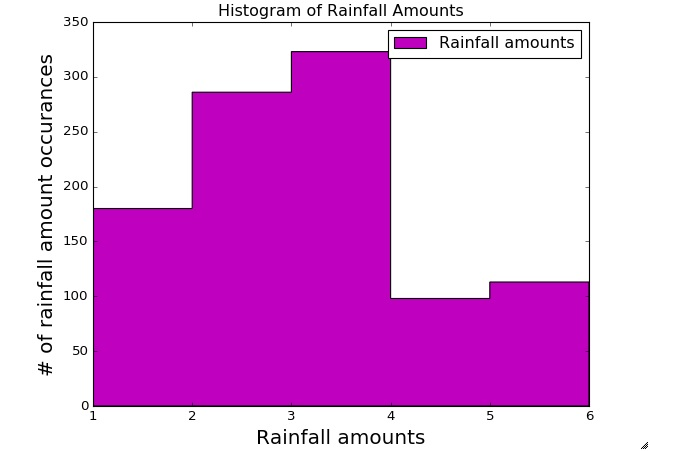
\includegraphics[width=0.5\textwidth]{Histogram.jpg}
	\caption{\it This is a picture of the histogram that I created. \label{Histogram of Rainfall}}

\end{figure} 

{\it My histogram is showing the number of times that the rainfall amounts occur. Check it out in Fig.~\ref{Histogram of Rainfall}


%%%%%%%%%%%%%%%%%%%%%%%%%%%%%%%%%%%%%%%%%%%%%%%%%%%%%%%%%%%%%%%%%%%%%%%%%%%%%%%%
\end{document}
%%%%%%%%%%%%%%%%%%%%%%%%%%%%%%%%%%%%%%%%%%%%%%%%%%%%%%%%%%%%%%%%%%%%%%%%%%%%%%%%
